\documentclass[a4paper, doc, natbib]{apa6}

\usepackage[english]{babel}
\usepackage[utf8x]{inputenc}
\usepackage{amsmath}
\usepackage{graphicx}
\usepackage[colorinlistoftodos]{todonotes}
\usepackage{glossaries}

\addto\captionsenglish{\renewcommand{\figurename}{Şekil.}}
\addto\captionsenglish{\renewcommand{\contentsname}{İÇİNDEKİLER}}

\addto\captionsenglish{\renewcommand{\listtablename}{Tablolar Listesi}}
\addto\captionsenglish{\renewcommand{\listfigurename}{Şekiller Listesi}}

\addto{\captionsenglish}{\renewcommand{\refname}{Kaynakça}}
\usepackage[tablename=Tablo.]{caption}



\makeglossaries
 
\newglossaryentry{ESA}
{
    name=ESA,
    description={Evrişimsel Sinir Ağları, Convolutional Neural Networks}
}
\newglossaryentry{BCE}
{
    name=BCE,
    description={İkili Çapraz Entropi, Binary Cross Entropy}
}


\title{Yazının Başlığı}
\shorttitle{ Kısa Başlık, sayfa üstünde gösterilir}
\author{Uğur Uysal, Yazarın Bilgileri}
\affiliation{İTÜ, Yazarın kurumu}

\begin{document}
\begin{titlepage}
    \maketitle
\end{titlepage}

\pagenumbering{Roman}

\tableofcontents
\newpage
\listoffigures
\newpage
\listoftables
\newpage
\printglossary[title={Kısaltmalar ve Simgeler Listesi}]
\newpage


\section*{Özet}

Burada yazının özet bölümü yer alır.
\newpage

\pagenumbering{arabic}
\section{GİRİŞ}
 Burada yazının giriş bölümüdür.
 Bu konuda öncül çalışmalar 1970li yıllarında \cite{Bajcsy1976ComputerRO} and Idelsohn \citep{terrain_recognition} tarafından yapılmıştır.

Burada atıf örneği görebilirsiniz.

\subsection{Motivasyon}
Çalışmanın temelindeki hedefler ve motivasyon. .

\subsection{Proje Özeti}
Makinalar öğrendi . .
\subsection{Veri Kümesi}
MINST veri kümesi . . 


\subsection{Yöntemler}
Yöntemlerin kısa özeti.

\clearpage
\newpage
\section{YÖNTEM VE TEKNİKLER}

\subsection{Öncül Çalışmalar}
Literatürdeki öncül çalışmalar. 


\subsection{Yöntemler}
Çalımadan kullanılan yöntemler detaylı anlatılır. 
\subsection{Objektif Fonksiyonları}

Örnek matematil denklemi.. Glassory örneği

\begin{equation}
    \text{\GLS{BCE}} = - \frac{1}{N}\sum_{i=0}^{N} y_i * log(\hat{y}_i) + (1-y_i)*log(1-\hat{y}_i) 
\end{equation}



\subsection{Ayrıntılı Veri Kümesi İncelemesi}
Veri kümesinin özellikleri. 


\subsection{Deney Detayları}
Deneylerin detayları..

\subsection{Değerlendirme Kriterleri}
Makine öğrenmesi algoritmalarının performanslarını değerlendirmek için çeşitli metrikler vardır. Bunlardan "doğruluk" ölçütü en sık karşımıza çıkandır. Yaygın olarak kullanılan değerlendirme kriterleri aşağıda verilmiştir. 

\begin{center}
    Accuracy = $\frac{TP + TN }{ TP + TN + FP + FN}$
\end{center}
\begin{center}
    Recall = $\frac{TP  }{ TP + FN}$
\end{center}
\begin{center}
    Precision = $\frac{TP }{ TP + FP}$
\end{center}
\begin{center}
    Dice Score = $\frac{ 2*TP }{ 2*TP + FP + FN}$
\end{center}
\begin{center}
    Intersection over Union = $\frac{ TP }{ TP + FP + FN}$
\end{center}

TP gerçek pozitif, TN gerçek negatif, FN yalancı negatif ve  FP yalancı pozitif olacak şekilde kısaltmalar kullanılmıştır. 

Nesne tespit ya da anlamsal bölütleme problemlerinde kesişimin birleşimine oranı metrik olarak kullanılmaktadır. Birden fazla sınıf olan problemlerde ortalama IoU skoru kullanılır. 
\begin{center}
    mIoU =  $\frac{1}{c} \sum_{i=0}^{c} \frac{ TP_i }{ TP_i + FP_i + FN_i }$ 
\end{center}

\begin{equation}
    C = 1 - \frac{1}{N} \sum min(1,\frac{ | L(a,b) * L(a',b') | } {L(a,b)} )
\end{equation}


\begin{figure}[ht!]
 \centering
 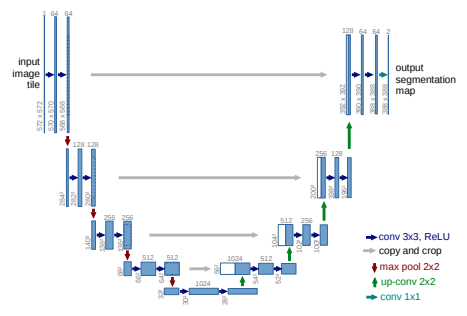
\includegraphics[width=0.9\linewidth]{ssunet.png}
 \caption{ Şekil örneği, U-Net }
 \label{figure:linknetmine}
\end{figure}

\clearpage
\newpage
\section{BULGULAR}
\subsection{Deneyler}
Bu çalışmadan yapılan deneyler aşağıda Tablo \ref{table:experiments}'de verilmiştir. Burada metin içinde tabloya referens örneği görmektesinz.

\begin{table}[ht]
 \begin{center}
  \begin{tabular}{|l|c|c|}
   \hline
   Sütun1 & Sütun2 & Sütun3 \\
   \hline\hline
   Değerler  &  Değerler  & Değerler \\
   \hline
   Değerler  &  Değerler & 4 \\
   \hline
   Değerler  & Değerler & 8 \\
   \hline
   Değerler  & Değerler & 6 \\
   \hline
   Değerler  & Değerler & 6 \\
   \hline
   Değerler  & Değerler & 6 \\
   \hline
  \end{tabular}
 \end{center}
 \caption{Tablo Örneği  }
 \label{table:experiments}
\end{table}


\begin{figure}[ht!]
 \centering
  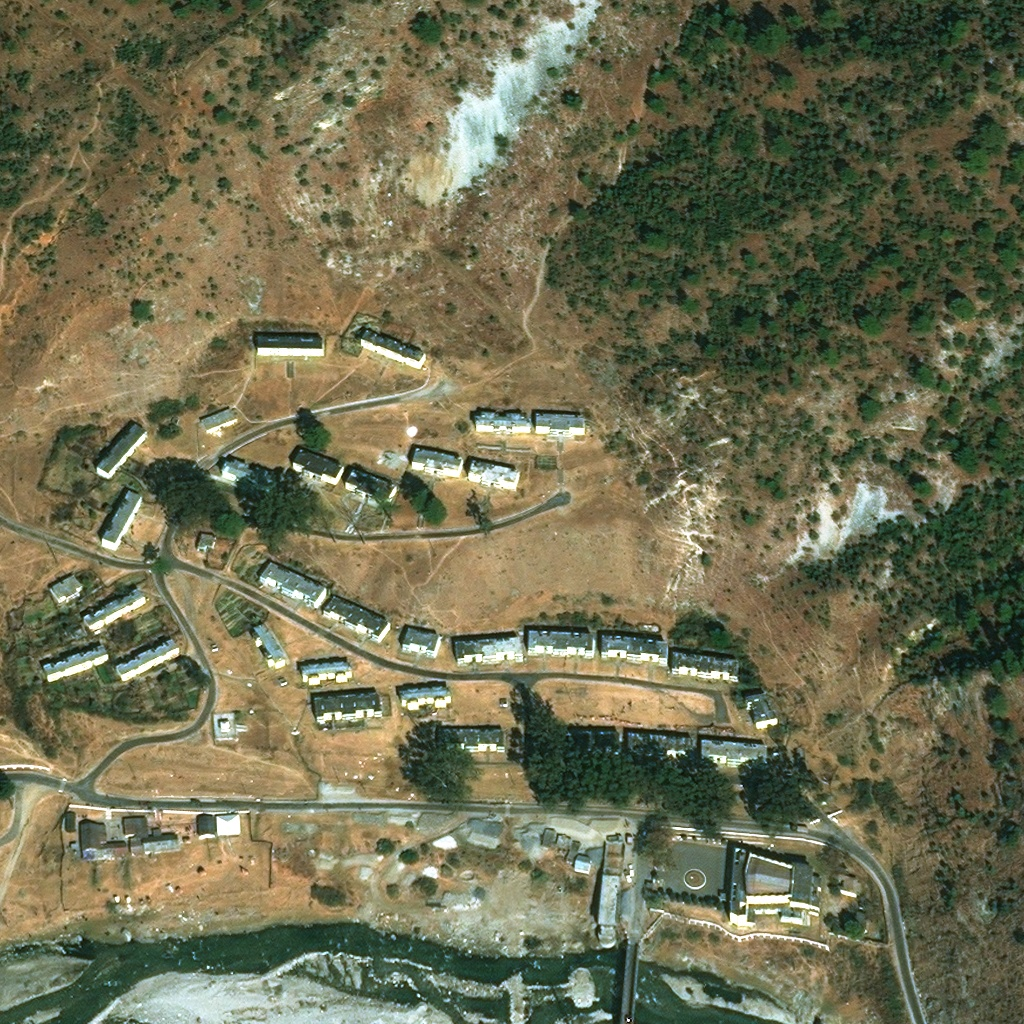
\includegraphics[width=0.25\linewidth]{sat/1392_sat.jpg}
   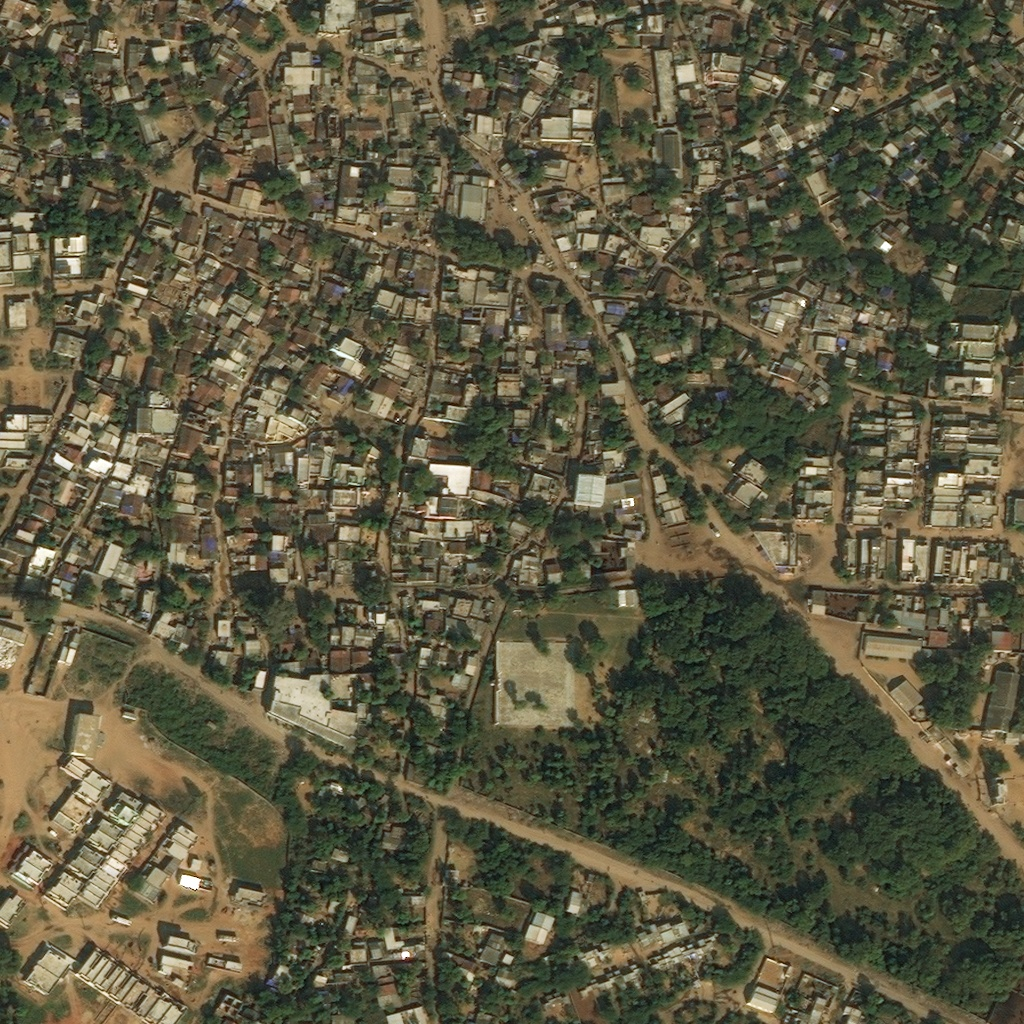
\includegraphics[width=0.25\linewidth]{sat/9821_sat.jpg}
     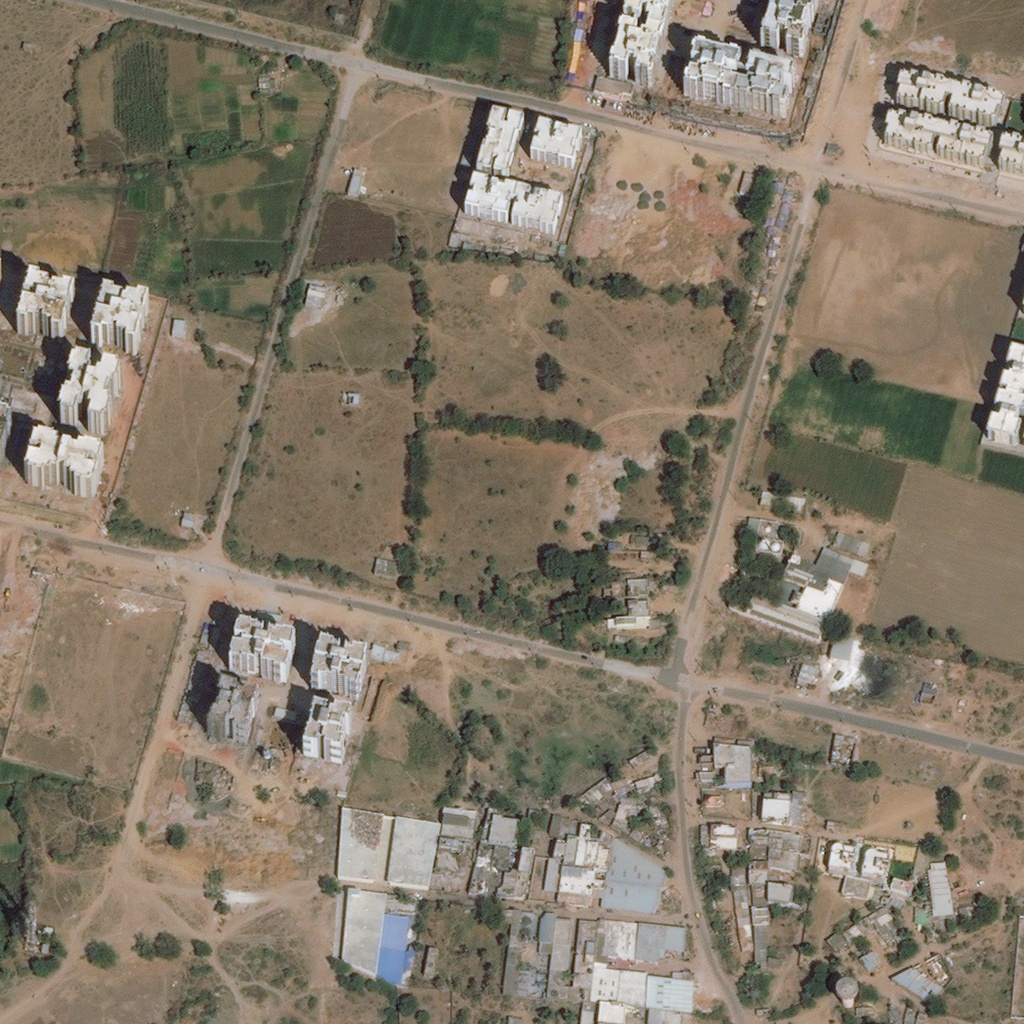
\includegraphics[width=0.25\linewidth]{sat/290434_sat.jpg}
 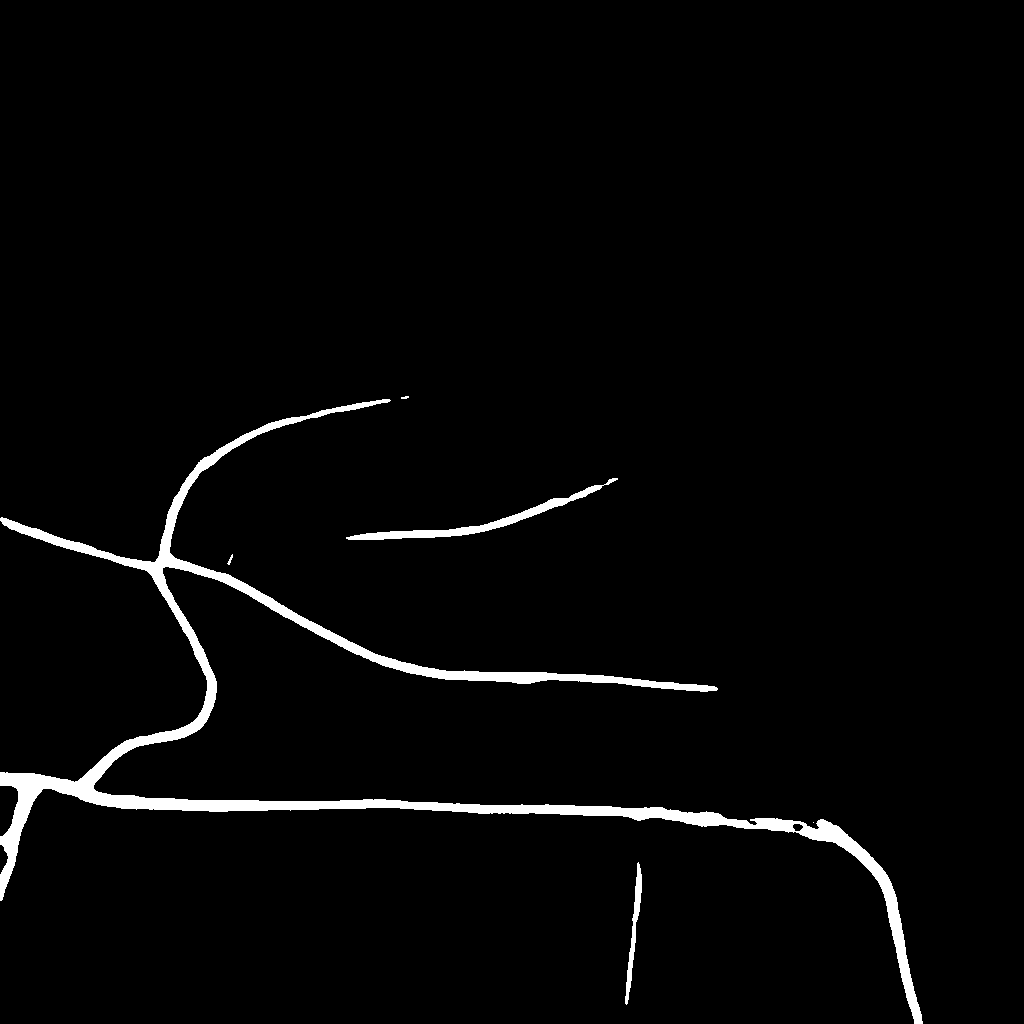
\includegraphics[width=0.25\linewidth]{l1/l1_1392_mask.png}
  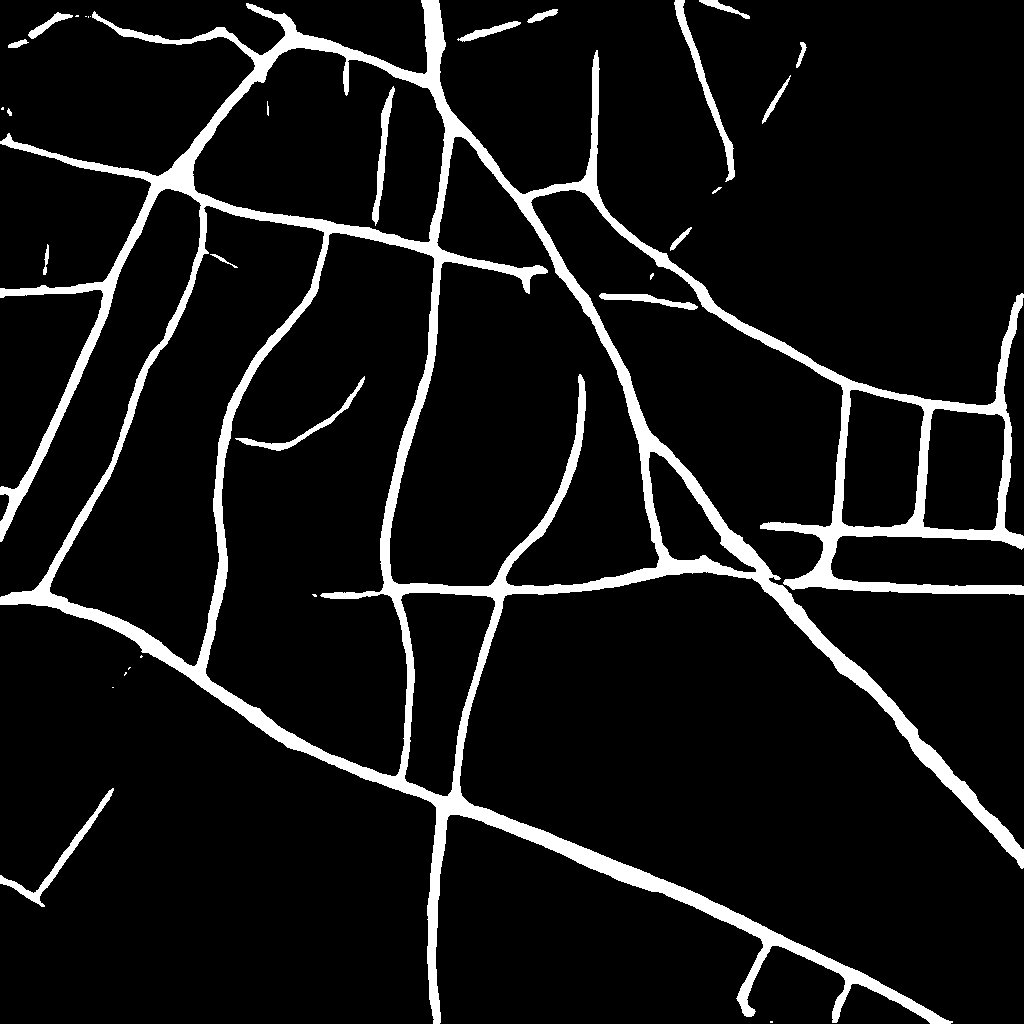
\includegraphics[width=0.25\linewidth]{l1/l1_9821_mask.png}
    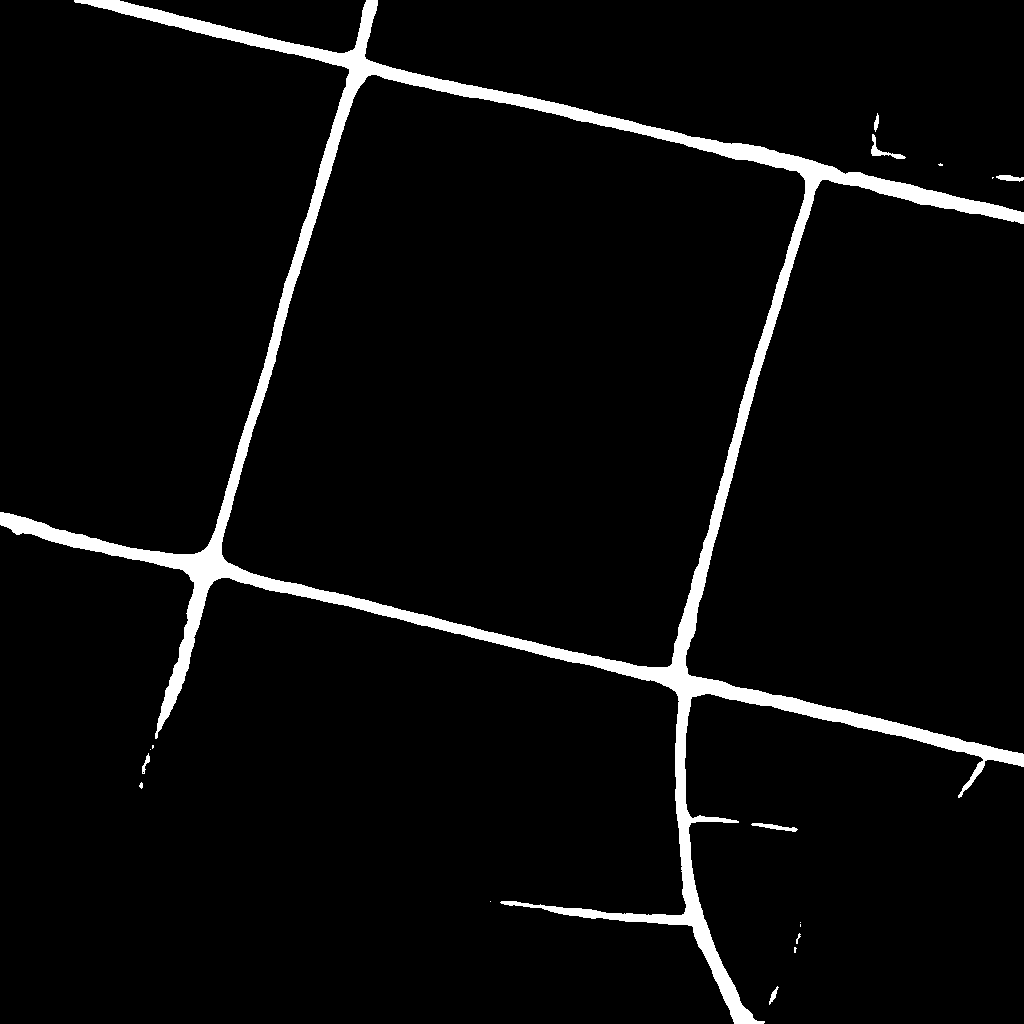
\includegraphics[width=0.25\linewidth]{l1/l1_290434_mask.png}
 \caption{ Figürlerin karışık  }
 \label{figure:secondexper}
\end{figure}

\clearpage
\newpage
Boş sayfa 
\clearpage
\newpage
\subsection{Toplu Nitel Sonuçlar}

\clearpage
\newpage
\section{Sonuç ve Tartışma}

\clearpage
\bibliography{example}
\end{document}

%
% Please see the package documentation for more informatclass:
%
% http://www.ctan.org/pkg/apa6
%olut et. al.